\documentclass[a4, 11pt]{article}

% #####################################################################################################################
\usepackage[utf8]{inputenc}
\usepackage[a4paper]{geometry}
\geometry{verbose,tmargin=4cm,bmargin=2.5cm,lmargin=2cm,rmargin=2cm,headheight=0.8cm,headsep=1cm,footskip=0.5cm}
\pagestyle{headings}
\setcounter{secnumdepth}{3}
\usepackage{url}
\usepackage{graphicx}
\usepackage{setspace}
% ############################################################################
% ############## Packages and Newcommands defined for AG #####################
% ############################################################################
\newcommand\hmmax{0}		% AG: odstraneni omezeni na pocet pouzitych fontu, obzvlast v AMS
\newcommand\bmmax{0}		% AG: odstraneni omezeni na pocet pouzitych fontu, obzvlast v AMS

\usepackage{amsfonts, amssymb, amsmath, amstext, amsthm}	        % math
\usepackage{physics}												% physics
\usepackage{braket}
\usepackage{esvect}                                                 % vectors with arrow, cmd is \vv{}
\usepackage{listings}		                                        % package for inserting codes
%\usepackage[framed,numbered,autolinebreaks,useliterate]{mcode}      % custom package in this dir, for m-code in latex
\usepackage{array, delarray}
\usepackage[utf8]{inputenc}                                         % english and also czech characters
\usepackage[czech]{babel}
\usepackage[IL2]{fontenc}                                           % zlepseni sazby v CZ. pripadne [T1], je to universalnejsi, nebo [IL2]
\usepackage{color, xcolor}                                          % defining package for some colors... also colors ("red", "green", etc.)
\usepackage{bm}
\usepackage{makeidx}                                                % makes index
\usepackage{hyperref}                                               % references
\usepackage{epstopdf, epsfig, graphicx}                             % pictures
\usepackage{blindtext, rotating}                                    % rotating images
\usepackage{epsfig}
\usepackage{float}                                                  % no floating figures in text anymore. Just add [H] behind begin figure!
\usepackage{booktabs, multirow}                                     % tables
\usepackage{hhline}
\usepackage{epigraph}                                               % citations
\usepackage{svg}		                                            % prime vkladani svg souboru

\usepackage{pdfpages}  												% prime vkladani pdf stranek pomoci prikazu \includepdf[pages=-]{myfile.pdf}
\usepackage{pgfplots}
%\usepackage{}
\usepackage[ddmmyyyy,hhmmss]{datetime}								% insert \today or \currenttime to see it
\usepackage{csquotes}
\usepackage{framed}

\usepackage{enumerate}
\usepackage[shortlabels]{enumitem}

\usepackage{shadethm}
\usepackage[stable]{footmisc}                                       % Load the footmisc package with the stable option

%\usepackage[scale=4.5, text=draft, color={[gray]{0.96}}]{draftwatermark}                                         % package for watermark 'draft' on each page


%\usepackage{watermark}                                         % package for watermarks  just add in document '\watermark{mytext}' and thats it.

%\usepackage[printwatermark]{xwatermark}

\usepackage{bm}

%%%%%%%%%%%%%%%%%%%%%%%%%%%%%%%%%%%%%%%%%%%%%%%%%%%%%%%%%%%%%%%%%%%%%
%% My unique commands in LaTeX
\newcommand{\ekviv}{ \Leftrightarrow }                           % ekvivalence (prave tehdy kdyz)
\newcommand{\commm}[1]{{\textcolor[cmyk]{0,1,0,0}{\textbf{\textsf{#1}}}}}      % new, commenting command, also red coloring
\newcommand{\com}[1]{\textbf{{\textsf{#1}}}}         % new, commenting command just comments
\newcommand\tab[1][1cm]{\hspace*{#1}}                % tabulator. tak jak ho zname z MS Wordu etc. 1cm
\newcommand{\slo}[1]{\medskip}                       % fakticky sloka pro verse
\newcommand{\uvoz}[1]{``{#1}''}                        % klasicke ENG uvozovky, vzdy funkcni... bylo drive {„{#1}“}

\newcommand{\chapquote}[3]{\begin{quotation} \textit{#1} \end{quotation} \begin{flushright} -- #2 \textit{#3}\end{flushright} }
% priklad na chapquote: \chapquote{Begin at the beginning,the King said gravely,and go on till you come to the end: then stop.}{Lewis Carroll}{Alice in Wonderland}
\renewcommand{\vec}[1]{\vv{#1}}  %{\boldsymbol{#1}}
\newcommand{\R}{ \ensuremath{\mathbb{R}} }

\newcommand{\setof}[1]{\ensuremath{\bm{\mathbf{#1}}}}				% mnozina prvku, vstup POUZE CAPSLOCK (funguje i na recka pismenka)
\newcommand{\alg}[1]{\ensuremath{\mathsf{#1}}}				% algebra 
\newcommand{\nv}[1]{\ensuremath{\mathcal{#1}}}			% nahodna velicina vstup POUZE CAPSLOCK
\newcommand{\deftxt}[1]{\textit{\textcolor{mygreen}{#1}}}			% nazev toho, co prave definuji (jen uvnitr definice)

\newcommand{\azar}{\ensuremath{  \land  }}			% symbol pro 'a zaroven'
\newcommand{\id}[1]{\ensuremath{  {}^I{#1}   }}				% velke I v predindexu, pro ideal v FPD

\newcommand{\oper}[1]{\ensuremath{\mbox{\textbf{\textsf{{\^{#1}}}}}}}				% operator (in QM or in general) ... bylo \mathsf{#1}
\newcommand{\mtx}[1]{\ensuremath{\mathbb{#1}}}

% Expectation symbol
\DeclareMathOperator*{\E}{\mathbb{E}}
% KLD operator
\DeclareMathOperator*{\KLD}{\mathrm{D}}

\renewcommand{\d}{\ensuremath{\mathrm{d}}}   % diferencial

\newcommand{\Hilsp}{ \ensuremath{\mathcal{H}}}   % Hilbert space

\newcommand{\dk}[1]{\begin{proof}#1\end{proof}}

\newcommand{\tequal}[1]{  \ensuremath{  \stackrel{\text{#1}}{=}  }  } % tequal{bla!} in math mode types equal sign with the specified text above it

% ######### helping to chop the words
\hyphenation{roz-ho-do-va-cích}
\hyphenation{Me-to-do-lo-gic-ky}
\hyphenation{for-ma-li-sa-tion}

% ######### defining my own colors
\definecolor{mygreen}{RGB}{3, 99, 50}   
\definecolor{myorange}{RGB}{3, 99, 50}

% ######### defining my math environmets
\theoremstyle{definition}
\newtheorem{definition}{Definition}{}


\newtheorem{temptheoforbackground}{Theorem}
\newenvironment{theorem}
{\colorlet{shadecolor}{green!15}
	\begin{shaded}  \vspace{-10pt}
		\begin{temptheoforbackground}
		}
		{
		\end{temptheoforbackground} \vspace{-10pt}
	\end{shaded}
}


\newtheorem{temppostulateforbackground}{Postulate}
\newenvironment{postulate}
{
	\colorlet{shadecolor}{orange!15}
	\begin{shaded} \vspace{-10pt}
		\begin{temppostulateforbackground}
		}
		{
		\end{temppostulateforbackground} \vspace{-10pt}
	\end{shaded}
}

\newtheorem{tempassumptionforbackground}{Assumption}
\newenvironment{assumption}
{
	\colorlet{shadecolor}{red!15}
	\begin{shaded} \vspace{-10pt}
		\begin{tempassumptionforbackground}
		}  
		{
		\end{tempassumptionforbackground} \vspace{-10pt}
	\end{shaded}
}



\theoremstyle{remark}
\newtheorem{remark}{Remark}{}

% ######### making index
\makeindex

%opening
\title{SKE protokol}

\author{Aleksej Gaj\footnote{email: \href{mailto:aleksejalex@gmail.com}{aleksejalex@gmail.com}}}

\begin{document}
	\maketitle	
	\tableofcontents
	
	\newpage
	
	\begin{postulate}[Jen pro mně: censored vs died]
		In the context of survival analysis, censored data refers to observations that are incomplete or not fully observed. Censoring occurs when the exact event time (such as death) for a subject is unknown or has not yet occurred at the end of the study or the time of analysis.
		
		In your dataset with patients, if the event of interest is whether they have died or not, the "censored" status indicates that the patient's event status is unknown because they were still alive or their follow-up time ended before the event occurred. It means that the patient was observed for a certain period but the event (death) did not occur within that period. Censoring can happen due to various reasons, such as the end of the study, loss to follow-up, or the patient being still alive at the time of analysis.
		
		In survival analysis, censored data is an important consideration. Statistical methods, like the Cox proportional hazards model or Kaplan-Meier estimator, handle censored data appropriately and use the available information to estimate survival probabilities and hazard rates.
		
		When analyzing your dataset, you would need to take into account both the "died" events and the censored observations to obtain valid estimates of survival probabilities or hazard ratios. The censored observations contribute information about the time the patient was followed until censoring, which is valuable in estimating the survival function beyond the observed events.
		
		It's crucial to appropriately handle and interpret censored data in survival analysis to obtain reliable conclusions about the survival experience of patients in your study.
	\end{postulate}
\newpage
	
	\section{Zadání}\label{sec:zadani}
	\textbf{A)} \textit{Pomocí parametrických a neparametrických metod pro cenzorovaná data odhadněte vhodný spolehlivostní model pro časy dožití (survt Tj) obou vybraných podskupin pacientů. Pro kontrolu fitu parametrické rodiny užijte Kaplan-Meierův plot nebo Nelson-Aalenův ‘hazard plot‘ (nejlépe v jednom obrázku spolu s parametrickým průběhem), resp. QQ/PP při RC.} \\
	\textbf{B)} \textit{SROVNEJTE tyto vybrané podskupiny vzhledem k jejich
	\begin{itemize}
		\item průběhu spolehlivosti (survival function) R(t), resp.
		\item intenzitě poruch (survivals) $ \lambda(t) $ (IFR/DFR/CFR), resp.
		\item kumulativní intenzitě poruch (survivals) $ \Lambda(t) $, resp.
		\item střední době života MTTF, resp.
		\item mediánové době života $ t_{med} $, resp.
		\item ...(jiné vlastní, pokud vás něco osloví)
	\end{itemize}} 
	\noindent
	\textbf{C)} \textit{Graficky srovnejte log-logR ploty pro obě podskupiny a na jejich základě zdůvodněte vhodnost/nevhodnost užití Coxova PH (proportional hazard) modelu.} \\
	\noindent
	\textbf{Skupina II.:}  treat=1(standard) versus treat=2(placebo) pro cell=2(small) \\
	
	\section{Dataset}\label{sec:dataset}
	Poskytnutý dataset představuje záznam testování vlivu jistého léčiva na dobu přežití pacienta. Data se skládají ze 137 pozorování 8 proměnných, viz Tabulka~\ref{tab:promenne_popis}. Cílem je modelovat dobu dožití (\textit{survival time}), tedy \texttt{survt} je vysvětlovaná proměnná.
	Ta je censorována podle proměnné \texttt{cens}. Další proměnné, které jsou k dispozici, představují věk pacienta, typ buněk, Karnofsky score (představující závažnost nemoci\footnote{Pozn: Hodnoty Karnofského skóre znamenají: $ KAR\leq30 $ -- úplná hospitalizace, $30<KAR\leq60$ -- částečná hospitalizace, $ KAR>60 $ -- vlastní péče bez hospitalizace.}), trvání nemoci (proměnná \texttt{didur}) a zda pacient už absolvoval léčbu v minulosti. 
	
	V této práci se zaměříme na skupinu pacientů s typem buněk \texttt{cell}=2. 
	
\begin{table}[H]
	\centering
	\begin{tabular}{@{}ll@{}}
		\toprule
		Název prom. & Komentář                    \\ 
		\midrule
		treat & treatment (1 = standard/lék, 2 = test/placebo)                    \\
		cell  & cell type (1 = squamous, 2 = small, 3 = adeno, 4 = large)         \\
		survt & survival time   (days)                                          \\
		cens  & status (0 = censored, 1 = died)                                 \\
		KAR   & performance status -- Karnofsky score (0 = worst,..., 100 = best) \\
		didur & disease duration from diagnosis to treatment (months)           \\
		age   & age (years)                                                     \\
		prith & prior therapy (0 = none, 10= some)                             \\
		\bottomrule
	\end{tabular}
	\caption{Popis proměnných v datasetu}
	\label{tab:promenne_popis}
\end{table}

V Tabulce~\ref{tab:zaklad_anal_cely_dataset} je uveden základní analýza na celém datasetu.

\begin{table}[H]
	\centering
	\begin{tabular}{lrrrrrrrr}
		\toprule
		& treat & cell & survt & cens & KAR & didur & age & prith \\
		\midrule
		count & 137.00 & 137.00 & 137.00 & 137.00 & 137.00 & 137.00 & 137.00 & 137.00 \\
		mean & 1.50 & 2.34 & 121.63 & 0.74 & 58.57 & 8.77 & 58.31 & 2.92 \\
		std & 0.50 & 1.07 & 157.82 & 0.44 & 20.04 & 10.61 & 10.54 & 4.56 \\
		min & 1.00 & 1.00 & 1.00 & 0.00 & 10.00 & 1.00 & 34.00 & 0.00 \\
		25\% & 1.00 & 1.00 & 25.00 & 0.00 & 40.00 & 3.00 & 51.00 & 0.00 \\
		50\% & 1.00 & 2.00 & 80.00 & 1.00 & 60.00 & 5.00 & 62.00 & 0.00 \\
		75\% & 2.00 & 3.00 & 144.00 & 1.00 & 75.00 & 11.00 & 66.00 & 10.00 \\
		max & 2.00 & 4.00 & 999.00 & 1.00 & 99.00 & 87.00 & 81.00 & 10.00 \\
		\bottomrule
	\end{tabular}
	\caption{Základní analýza na celém datasetu} \label{tab:zaklad_anal_cely_dataset}
\end{table}
	
	
	\subsection{Základní analýza}
	\commm{TODO: popis o co jde, tabulka describe celeho datasetu a mych dat}
	Cílem je zjistit, jak dané léčivo ovlivnilo dobu dožití pacientů v porovnání s placebem. 


\begin{table}[H]
	\centering
\begin{tabular}{lrrrrrrrr}
	\toprule
	& treat & cell & survt & cens & KAR & didur & age & prith \\
	\midrule
	count & 48.00 & 48.00 & 48.00 & 48.00 & 48.00 & 48.00 & 48.00 & 48.00 \\
	mean & 1.38 & 2.00 & 71.67 & 0.75 & 53.54 & 9.25 & 59.88 & 2.29 \\
	std & 0.49 & 0.00 & 85.77 & 0.44 & 19.10 & 13.91 & 9.92 & 4.25 \\
	min & 1.00 & 2.00 & 2.00 & 0.00 & 20.00 & 1.00 & 35.00 & 0.00 \\
	25\% & 1.00 & 2.00 & 20.00 & 0.75 & 40.00 & 2.00 & 54.75 & 0.00 \\
	50\% & 1.00 & 2.00 & 51.00 & 1.00 & 60.00 & 4.00 & 62.50 & 0.00 \\
	75\% & 2.00 & 2.00 & 97.50 & 1.00 & 70.00 & 11.00 & 67.00 & 0.00 \\
	max & 2.00 & 2.00 & 392.00 & 1.00 & 85.00 & 87.00 & 72.00 & 10.00 \\
	\bottomrule
\end{tabular}
	\caption{Základní analýza na podvybraném datasetu ($\mbox{\texttt{cell}}=2$)}
\end{table}


	
	\subsection{Vizualizace}
	\commm{TODO: histogram, boxplot}
	
\begin{figure}[H]
	\centering
	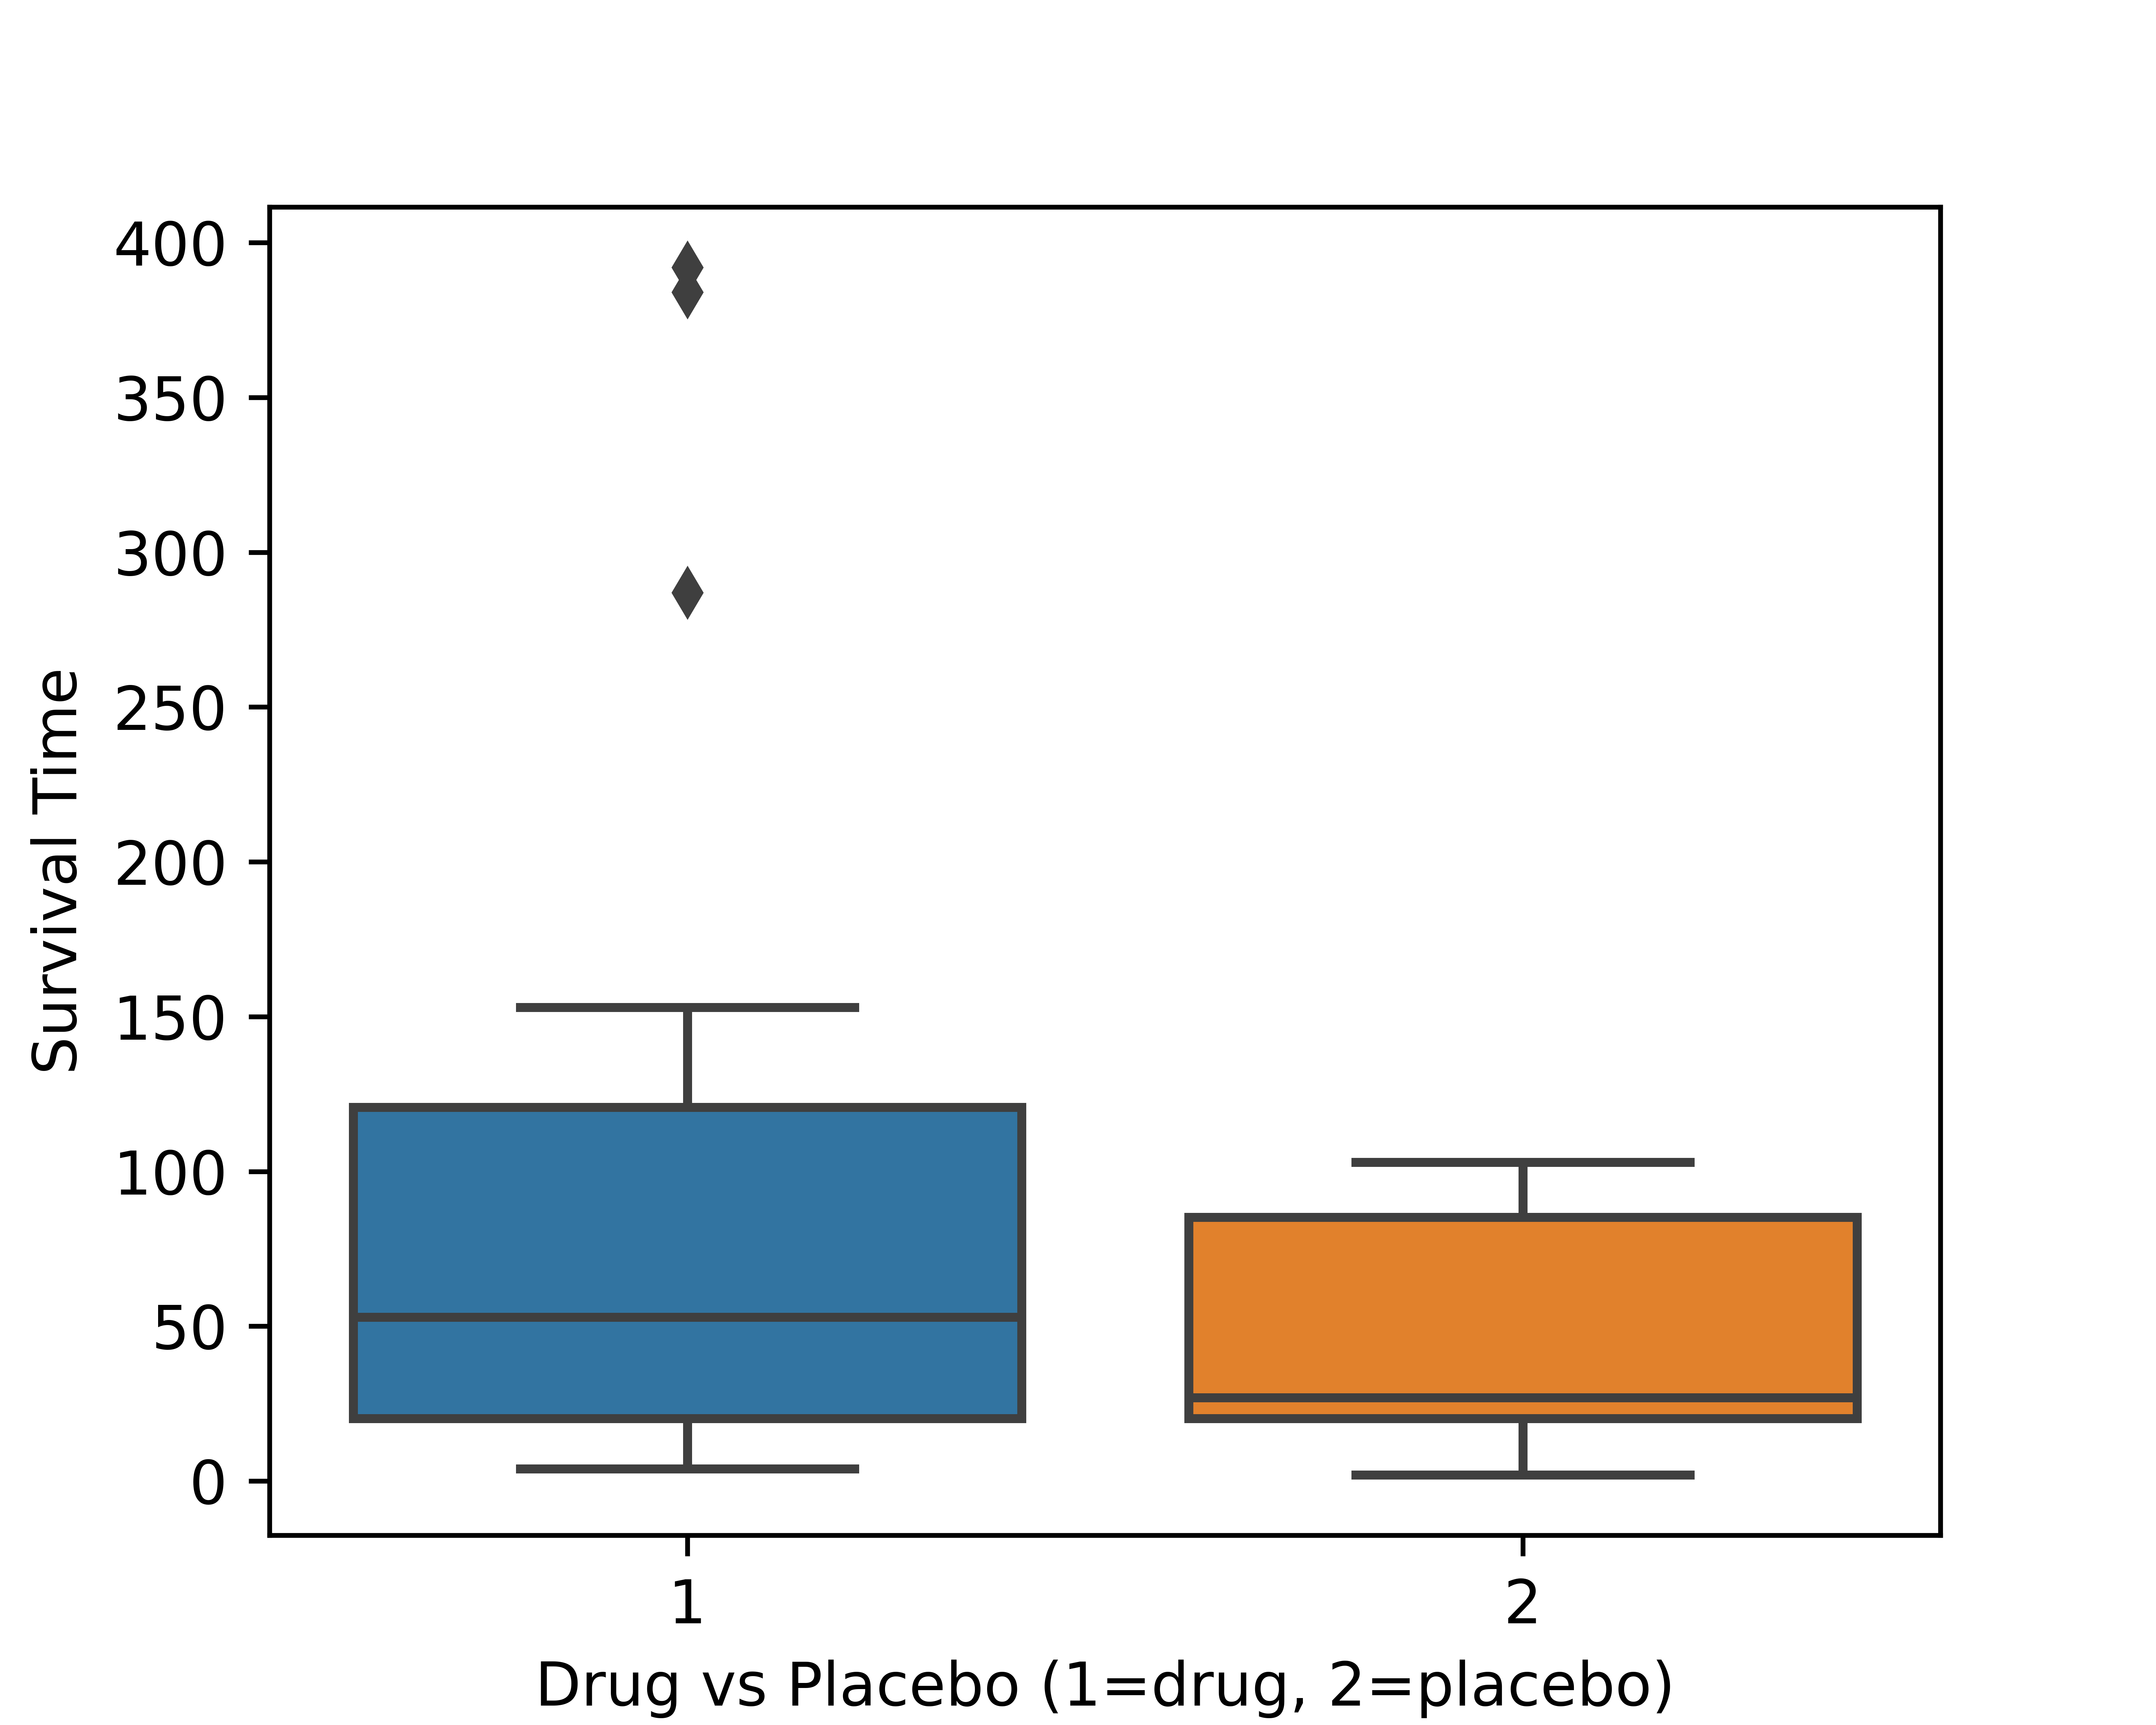
\includegraphics[width=0.7\linewidth]{img/boxplot_drug_vs_placebo}
	\caption[Boxplot doby dožití]{Boxplot doby dožití}
	\label{fig:boxplotdrugvsplacebo}
\end{figure}





	\section{Parametrické a neparametrické modely}
	\commm{TODO: balicek reliability}
	
	\section{Porovnání podskupin lék vs. placebo}
	
	\section{Coxův regresní model}
	\textit{Coxův regresní model} je založen na Coxově proporcionálním hazardovém předpokladu, který říká, že poměrné riziko dvou jedinců je konstantní v čase. Tento předpoklad umožňuje odhadnout vliv různých faktorů na přežití a současně zachovává nezávislost na neovlivňujících proměnných.
	
	Pro použití Coxova regresního modelu je nejprve potřeba mít k dispozici data o čase do události (např. úmrtí) a příslušné prediktory (faktory ovlivňující přežití). Zde byla použita existující implementace Coxova regresního modelu v knihovně \texttt{lifelines}.
	
	\subsection{Ověření předpokladů}

	\subsection{Model}
	
	
	\section{Závěr}\label{sec:zaver}
	We co

\end{document}